\documentclass[10pt]{amsart}

\usepackage{url}
\usepackage{tikz}
\usetikzlibrary{decorations.markings}
\usetikzlibrary{arrows,shapes,positioning}
\usepackage{calc}
\usepackage[compact]{titlesec}
\usepackage{caption}
\usepackage[labelformat=simple,labelfont={}]{subcaption}
\usepackage[margin=1in]{geometry} 
\usepackage{fancyhdr}
\usepackage{amsmath}
\usepackage{amsthm}
\usepackage{amssymb}
\usepackage{mathtools}
\usepackage{enumitem}
\usepackage{graphicx}
\usepackage{color}
\definecolor{darkblue}{rgb}{0, 0, .6}
\definecolor{grey}{rgb}{.7, .7, .7}
\usepackage[breaklinks]{hyperref}
\hypersetup{
	colorlinks=true,
	linkcolor=darkblue,
	anchorcolor=darkblue,
	citecolor=darkblue,
	pagecolor=darkblue,
	urlcolor=darkblue,
	pdftitle={},
	pdfauthor={}
}

\newcommand{\alert}[1]{\textcolor{darkblue}{\textbf{#1}}}

\begin{document}

\title{\alert{T-avoiding elements of Coxeter groups}}
\author{Thesis Proposal for Taryn Laird\\
Directed by Dana C.~Ernst}
 
\maketitle

A \alert{Coxeter system} is pair $(W,S)$ consisting of a distinguished (finite) set $S$ of generating involutions and a group $W$, called a \alert{Coxeter group}, with presentation
\[
W = \langle S \mid (st)^{m(s, t)} = e \text{ for } m(s, t) < \infty \rangle,
\]
where $e$ is the identity, $m(s,t) = 1$ if and only if $s = t$, and $m(s,t) = m(t,s)$. It turns out that the elements of $S$ are distinct as group elements, and that $m(s, t)$ is the order of $st$.  Since the elements of $S$ have order two, the relation $(st)^{m(s,t)} = e$ can be written as
\[
\underbrace{sts \cdots}_{m(s,t)} = \underbrace{tst \cdots}_{m(s,t)}
\]
with $m(s,t) \geq 2$ factors on each side of the equation.

Given a Coxeter system $(W,S)$, a word $s_{x_1}s_{x_2}\cdots s_{x_m}$ in the free monoid $S^*$ is called an \alert{expression} for $w\in W$ if it is equal to $w$ when considered as a group element. If $m$ is minimal among all expressions for $w$, the corresponding word is called a \alert{reduced expression} for $w$. In this case, we define the \alert{length} of $w$ to be $\ell(w)=m$. Each element $w \in W$ can have several different reduced expressions that represent it.  A product $w_{1}w_{2}\cdots w_{r}$ with $w_{i} \in W$ is called \alert{reduced} if $\ell(w_{1}w_{2}\cdots w_{r})=\sum \ell(w_{i})$.

Given a Coxeter system $(W,S)$, the associated \alert{Coxeter graph} is the graph $\Gamma$ with vertex set $S$ and edges $\{s,t\}$ labeled with $m(s,t)$ for all $m(s,t)\geq 3$.  If $m(s,t)=3$, it is customary to leave the corresponding edge unlabeled.  Given a Coxeter graph $\Gamma$, we can uniquely reconstruct the corresponding Coxeter system $(W,S)$.  In this case, we say that $(W,S)$, or just $W$, is of type $\Gamma$. If $(W,S)$ is of type $\Gamma$, for emphasis, we may write $W$ and $S$ as $W(\Gamma)$ and $S(\Gamma)$, respectively.  Note that generators $s$ and $t$ are connected by an edge in the Coxeter graph $\Gamma$ if and only if $s$ and $t$ do not commute. 

A few of the well-known Coxeter graphs are given in Figure~\ref{fig:CoxeterGraphs}. As an example, consider the Coxeter graph of type $A_n$. This determines the Coxeter system $(W(A_n),S(A_n))$ having $S(A_n) = \{s_1, s_2, \ldots, s_n\}$ as the distinguished generating set and defining relations
\begin{enumerate}
\item $s_is_i = e$ for all $i$;
\item $s_is_j = s_js_i$ when $|i-j| > 1$;
\item $s_is_js_i = s_js_is_j$ when $|i-j| = 1$.
\end{enumerate}
The Coxeter group $W(A_n)$ is isomorphic to the symmetric group $S_{n+1}$ under the correspondence $s_i\mapsto (i,i+1)$.

\begin{figure}[h!]
\centering
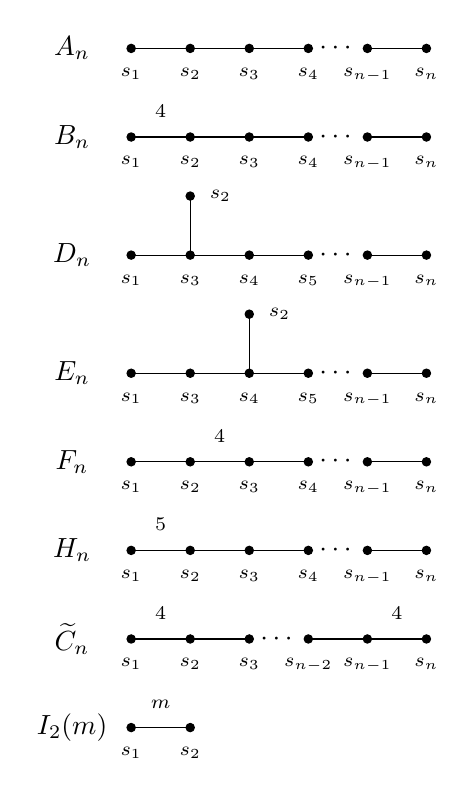
\begin{tikzpicture}[scale=.75]
%A_{n}
\draw[fill=black] \foreach \x in {1,2,...,6} {(\x,10) circle (2pt)};
\draw {(0,10) node{$A_{n}$}
\foreach \x in {1,2,...,4} {(\x,10) node[label=below:\scriptsize$s_{\x}$]{}}
(5,10) node[label=below:\scriptsize$s_{n-1}$]{}
(6,10) node[label=below:\scriptsize$s_{n}$]{}
(4.5,10) node{$\cdots$}
[-] (1,10) -- (4,10)
[-] (5,10) -- (6,10)}; 

%B_{n}
\draw [fill=black] \foreach \x in {1,2,...,6} {(\x,8.5) circle (2pt)};
\draw {(0,8.5) node{$B_{n}$}
\foreach \x in {1,2,...,4} {(\x,8.5) node[label=below:\scriptsize$s_{\x}$]{}}
(5,8.5) node[label=below:\scriptsize$s_{n-1}$]{}
(6,8.5) node[label=below:\scriptsize$s_{n}$]{}
(1.5,8.5) node[label=above:\scriptsize$4$]{}
(4.5,8.5) node{$\cdots$}
[-] (1,8.5) -- (4,8.5)
[-] (5,8.5) -- (6,8.5)}; 

%D_{n}
\draw[fill=black] \foreach \x in {1,2,...,6} {(\x,6.5) circle (2pt)};
\draw[fill=black] (2,7.5) circle (2pt);
\draw {(0,6.5) node{$D_{n}$}
(1,6.5) node[label=below:\scriptsize$s_{1}$]{}
(2,7.5) node[label=right:\scriptsize$s_{2}$]{}
(2,6.5) node[label=below:\scriptsize$s_{3}$]{}
(3,6.5) node[label=below:\scriptsize$s_{4}$]{}
(4,6.5) node[label=below:\scriptsize$s_{5}$]{}
(5,6.5) node[label=below:\scriptsize$s_{n-1}$]{}
(6,6.5) node[label=below:\scriptsize$s_{n}$]{}
(4.5,6.5) node{$\cdots$}
[-] (1,6.5) -- (4,6.5)
[-] (5,6.5) -- (6,6.5)
[-] (2,6.5) -- (2,7.5)}; 

%E_{n}
\draw[fill=black] \foreach \x in {1,2,...,6} {(\x,4.5) circle (2pt)};
\draw[fill=black] (3,5.5) circle (2pt);
\draw {(0,4.5) node{$E_{n}$}
(1,4.5) node[label=below:\scriptsize$s_{1}$]{}
(3,5.5) node[label=right:\scriptsize$s_{2}$]{}
(2,4.5) node[label=below:\scriptsize$s_{3}$]{}
(3,4.5) node[label=below:\scriptsize$s_{4}$]{}
(4,4.5) node[label=below:\scriptsize$s_{5}$]{}
(5,4.5) node[label=below:\scriptsize$s_{n-1}$]{}
(6,4.5) node[label=below:\scriptsize$s_{n}$]{}
(4.5,4.5) node{$\cdots$}
[-] (1,4.5) -- (4,4.5)
[-] (5,4.5) -- (6,4.5)
[-] (3,4.5) -- (3,5.5)}; 

%F_{n}
\draw[fill=black] \foreach \x in {1,2,...,6} {(\x,3) circle (2pt)};
\draw {(0,3) node{$F_{n}$}
\foreach \x in {1,2,...,4} {(\x,3) node[label=below:\scriptsize$s_{\x}$]{}}
(5,3) node[label=below:\scriptsize$s_{n-1}$]{}
(6,3) node[label=below:\scriptsize$s_{n}$]{}
(2.5,3) node[label=above:\scriptsize$4$]{}
(4.5,3) node{$\cdots$}
[-] (1,3) -- (4,3)
[-] (5,3) -- (6,3)}; 

%H_{n}
\draw[fill=black] \foreach \x in {1,2,...,6} {(\x,1.5) circle (2pt)};
\draw {(0,1.5) node{$H_{n}$}
\foreach \x in {1,2,...,4} {(\x,1.5) node[label=below:\scriptsize$s_{\x}$]{}}
(5,1.5) node[label=below:\scriptsize$s_{n-1}$]{}
(6,1.5) node[label=below:\scriptsize$s_{n}$]{}
(1.5,1.5) node[label=above:\scriptsize$5$]{}
(4.5,1.5) node{$\cdots$}
[-] (1,1.5) -- (4,1.5)
[-] (5,1.5) -- (6,1.5)}; 

%affineC_{n}
\draw[fill=black] \foreach \x in {1,2,...,6} {(\x,0) circle (2pt)};
\draw {(0,0) node{$\widetilde{C}_{n}$}
\foreach \x in {1,2,3} {(\x,0) node[label=below:\scriptsize$s_{\x}$]{}}
(4,0) node[label=below:\scriptsize$s_{n-2}$]{}
(5,0) node[label=below:\scriptsize$s_{n-1}$]{}
(6,0) node[label=below:\scriptsize$s_{n}$]{}
(1.5,0) node[label=above:\scriptsize$4$]{}
(5.5,0) node[label=above:\scriptsize$4$]{}
(3.5,0) node{$\cdots$}
[-] (1,0) -- (3,0)
[-] (4,0) -- (6,0)}; 

%I_{2}(m)
\draw[fill=black] \foreach \x in {1,2} {(\x,-1.5) circle (2pt)};
\draw {(0,-1.5) node{$I_{2}(m)$}
\foreach \x in {1,2} {(\x,-1.5) node[label=below:\scriptsize$s_{\x}$]{}}
(1.5,-1.5) node[label=above:\scriptsize$m$]{}
[-] (1,-1.5) -- (2,-1.5)};
\end{tikzpicture}
\caption{Several well-known Coxeter graphs.}
\label{fig:CoxeterGraphs}
\end{figure}

Suppose $(W,S)$ is a Coxeter system.  We say that $w\in W$ has \alert{Property T} if and only if $w=stu$ or $w=uts$, where the product is reduced and $m(s,t) \geq 3$.  In other words, a Coxeter group element has Property T if it has a reduced expression that begin or ends with a product of non-commuting generators.  In turn, we say that $w$ is \alert{T-avoiding} if and only if $w$ does not have Property T.

It is clear that if $w$ is a product of commuting generators, then $w$ is T-avoiding. If $w$ is T-avoiding but not a product of commuting generators, then we say that $w$ is \alert{bad}.

The central focus of this thesis is to address the following questions:
\begin{enumerate}
\item Which Coxeter systems contain bad elements?
\item If a Coxeter system contains bad elements, what form do they take?
\end{enumerate}
In other words, we would like to classify the T-avoiding elements of Coxeter groups.  It is highly unlikely that we will attain a complete classification.  Instead, we will take an ad hoc approach by studying specific Coxeter systems in turn.

We will now briefly summarize what is currently known about T-avoiding elements.  During the 2010--2011 academic year, D.C.~Ernst mentored J.~Cormier, Z.~Goldenberg, J.~Kelly, and C.~Malbon at Plymouth State University on a research project aimed at exploring the T-avoiding elements in Coxeter systems of types $A_n$ and $B_n$.  The research team discovered that there are no bad elements in either system.  That is, the only T-avoiding elements in Coxeter systems of types $A_n$ and $B_n$ are products of commuting generators.  In the case of type $A_n$, their results are a reformulation of known results, but with a much simpler proof.  Unfortunately, the students never finished writing up their results for publication and the proof in the case of type $B_n$ had been forgotten.  

During the 2011--2012 academic year, Ernst mentored R.~Cross, K.~Hills-Kimball, and C.~Quaranta at PSU on a project focused on the T-avoiding elements in Coxeter groups of type $F_n$.  In particular, the team successfully classified the T-avoiding elements in the infinite Coxeter system of type $F_{5}$, as well as the finite Coxeter system of type $F_{4}$. Both types included bad elements. At the time, the students conjectured that their classification holds more generally for arbitrary $F_{n}$.

In the Spring of 2013, Ernst worked with S.~Gilbertson at Northern Arizona University on extending the results obtained by Cross, Hills-Kimball, and Quaranta the previous year.  The initial goal was to prove that there were no new T-avoiding elements (other than multiplying by products of commuting generators) in type $F_n$ for $n\geq 6$.  However, Gilbertson discovered that this is horribly wrong.  It appears that the classification of T-avoiding elements in higher ranks gets more and more complicated.  Gilbertson and Ernst conjectured a classification of the T-avoiding elements in type $F_6$, but were unable to complete the proof.  The problem remains open.

In his PhD thesis, T.~Gern classified the T-avoiding elements in Coxeter groups of type $D_n$. Unlike in types $A_n$ and $B_n$, it turns out that the classification in type $D_n$ includes bad elements.

In the Spring of 2015, T.~Laird worked with Ernst on a semester-long research project involving T-avoiding elements of various Coxeter systems.  The major accomplishment of our work was the re-discovery of the proof of the classification of the T-avoiding elements in type $B_n$.  In addition, we conjectured a classification of the T-avoiding elements in Coxeter systems of type $\widetilde{C}_n$ and put most of the pieces of the proof together.

In this thesis, we propose to do the following.  First, we will summarize the currently known classifications of T-avoiding elements.  This will include our versions of the proofs for the classifications involving types $A_n$ and $B_n$.  Next, we will attempt to complete the proof of the classification in type $\widetilde{C}_n$. As time allows, we will tackle other Coxeter systems.  In particular, we will explore the T-avoiding elements in systems of type $E_n$ and see if we can make any additional headway in the case of type $F_n$.

\end{document}